\subsection{Training on Clips}

\begin{frame}[allowframebreaks]{Training on Clips: Key Considerations}
    \begin{itemize}
        \item \textbf{Clip Length Selection:} Typically, short clips of 16--64 frames are used to balance computational cost and temporal coverage.
        \item \textbf{Batch Size vs. Temporal Context:} Increasing clip length provides more temporal context but reduces the possible batch size due to memory constraints.
        \item \textbf{Pretraining for Transfer Learning:} Models are often pretrained on large-scale video datasets (e.g., Kinetics, Sports-1M) to improve performance on downstream tasks.
    \end{itemize}
\framebreak
    \begin{figure}
        \centering
        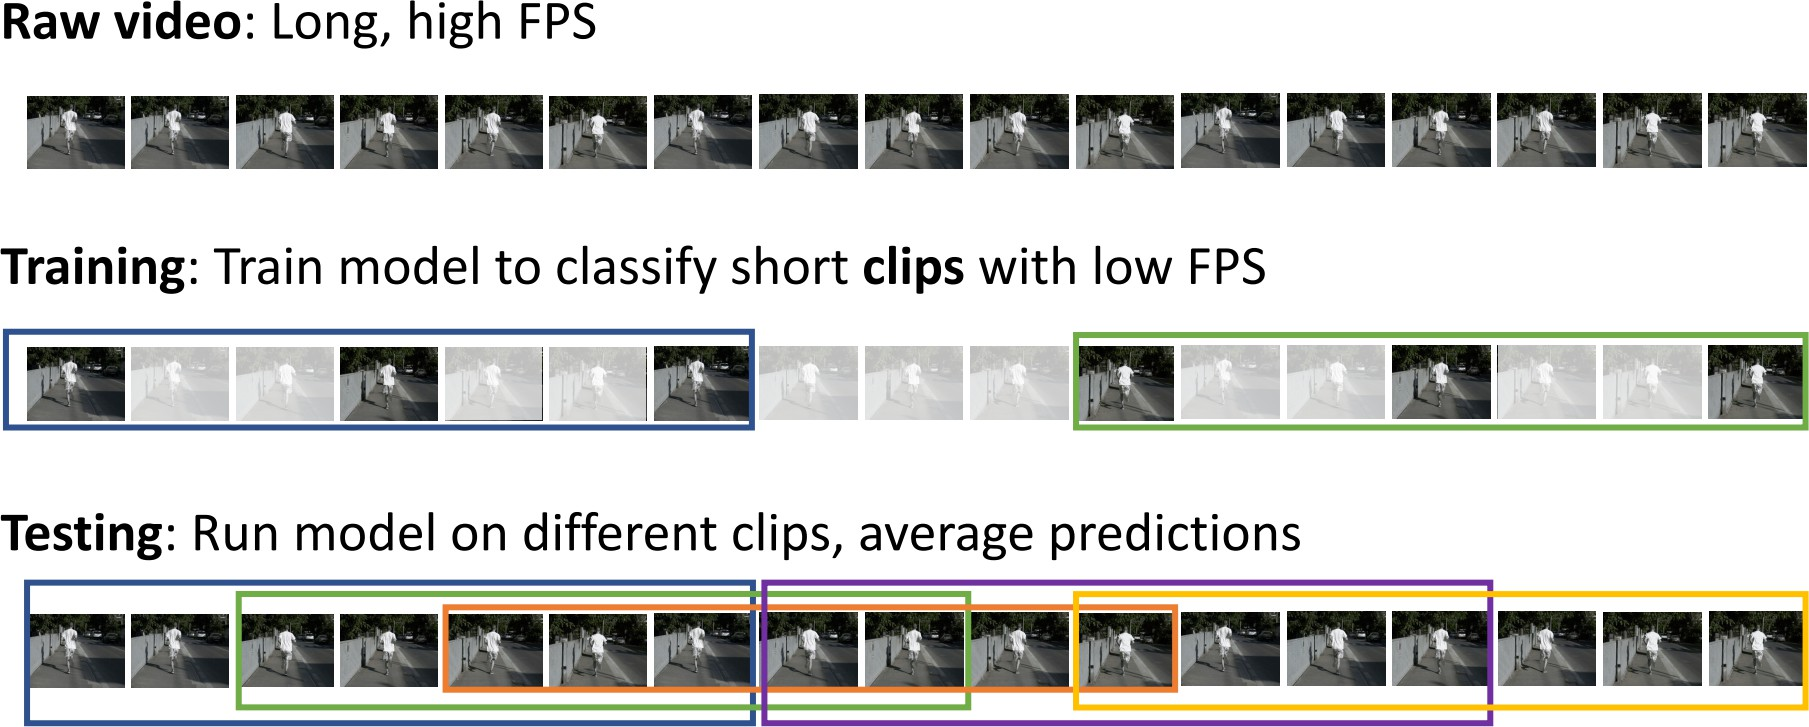
\includegraphics[width=1\textwidth,height=0.9\textheight,keepaspectratio]{images/video/slide_8_1_img.jpg}
    \end{figure}
\end{frame}